\documentclass[a4paper, 12pt]{article}
\usepackage[utf8]{inputenc}
\usepackage[brazil]{babel}
\usepackage{amstext} 	% need for \text command
\usepackage{amsmath}    % need for subequations
\usepackage{graphicx}   % need for figures
\usepackage{verbatim}   % useful for program listings
\usepackage{color}      % use if color is used in text
\usepackage{subfigure}  % use for side-by-side figures
\usepackage{hyperref}   % use for hypertext links, including those to external documents and URLs
\usepackage{pictexwd}	% use for pictex graphs
\usepackage{booktabs}	% use for Publication quality tables in LaTeX

%\author{Vítor M. Martins}
\title{PME2321}

\begin{document}
\maketitle
%\newpage
%\tableofcontents
%\newpage

\section{Ex 9.69 6ª Ed.}

\begin{figure}[h]
\begin{center}
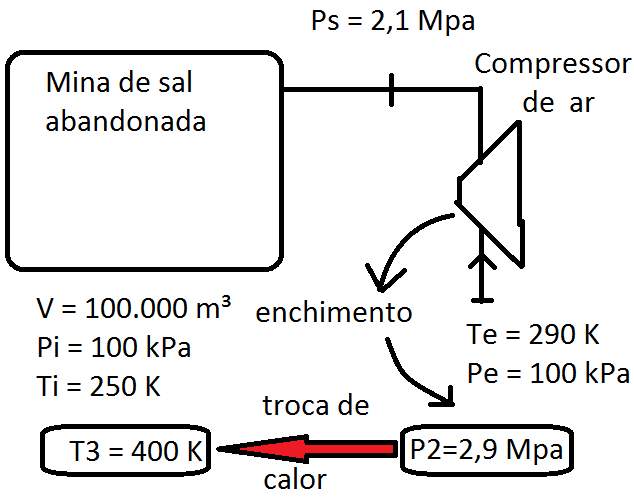
\includegraphics[scale=0.58]{./fig/1.png}
\caption{\label{fig:1}1} 
\end{center}
\end{figure}
\begin{itemize}
\item	a) $T_{2}=?$
\item	b) $m_{2}=?$
\item	c) $P_{3}=?$
\item	d) $T_{2 \rightarrow 3}=?$
\end{itemize}

\subsection*{Soluçao}

\subsubsection*{item a}

\paragraph*{Processo Transiente} (regime uniforme)
Volume de Controle $\rightarrow$ mina $+$ compressor

1ª Lei: 
\[m_{e}h_{e}=m_{2}u_{2}-m_{1}u_{1}+W_{c} \footnote{Trabalho do compressor}\]
\[m_{2}=m_{1}+m_{e}\]

2ª Lei: 
\[m_{2}s_{2}-m_{1}s_{1}=m_{e}s_{e}\]
\[s_{e}=s_{1}\]
\[m_{2}=m_{1}+m_{e}\]
\[s_{e}=s_{1}\]

\[s_{2}-s_{1}=0=(s_{T2}^{0}-s_{T1}^{0}-R\ln(\frac{P_{2}}{P_{1}}))\]
\[0=(s_{T2}^{0}-6.83512-0.287\ln(\frac{2100}{100}))\]
\[s_{T2}^{0}=7.709 \rightarrow T_{2} = 680 K\]

\subsubsection*{item b}
\[P_{2}V=m_{2}RT_{2}\]
\[m_{2}=1.0760*10^{6}kg\]

\subsubsection*{item c}
\[\frac{P_{2}}{T_{2}}=\frac{P_{3}}{T_{3}}\]
\[P_{3}=1235\ kPa\]

\subsubsection*{item d}
\paragraph*{Sistema}: 
\[Q_{2 \rightarrow 3}=U_{3}-U_{2}+W_{2 \rightarrow 3} \footnote{Trabalho nulo}\]
\[Q_{2 \rightarrow 3}=m_{2}(u_{3} \footnote{$u_{3}[T_{3}=400K]$} - u_{2} \footnote{$u_{2}[T_{2}=680K]$} )=-2.264*10^{8}kJ\]


\section{Ex 8.135}
\begin{figure}[h]
\begin{center}
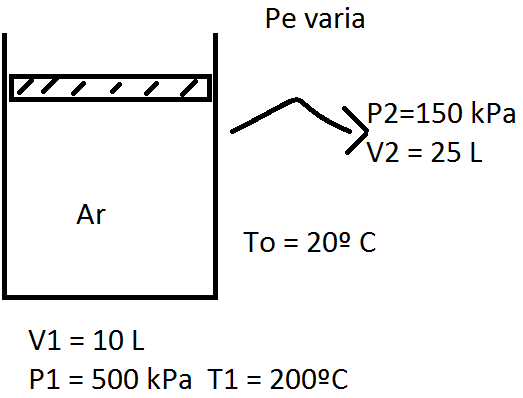
\includegraphics[scale=0.58]{./fig/2.png}
\caption{\label{fig:1}2} 
\end{center}
\end{figure}
\begin{itemize}
\item	a) $W=?$
\item	b) Isso é possível?

\end{itemize}

\subsection*{Soluçao}

\subsubsection*{item a}
\paragraph*{1ª Lei}  
\[Q_{1 \rightarrow 2S}=m_{2}u_{2S}-m_{1}u_{1}+W_{1 \rightarrow 2S}\]
\[W_{1 \rightarrow 2S}=mc_{V}(T_{1}-T_{2,S})\]
\paragraph*{2ª Lei (Adiabático e Reversível)}  
\[s_{2}-s_{1}=\frac{Q_{1 \rightarrow 2S}}{T}\]
Portanto: $s_{2}$=$s_{1}$
Hipótese: $c_{p}$ constante
\[\frac{T_{2,s}}{T_{1}}=(\frac{P_{2}}{P_{1}})^{\frac{k-1}{k}}\]
Portanto: $T_{2,S}$ = 335.3 K

\subsubsection*{item b}
Possível?

\[\Delta S_{liq} > 0\]
\[\Delta S_{liq} = (m_{2}s_{2}-m_{1}s_{1})\footnote{sistema} -  \frac{Q_{1 \rightarrow 2S}}{T_{0}}\footnote{meio}\]
\[\Delta S_{liq} = (0.002094) -  \frac{-0.5774}{293} = 0.004065 kJ/K\]
\[\Delta S_{liq}=m(s_{2}-s_{1})= m[c_{p}\ln(\frac{T_{2}}{T_{1}}) - R\ln(\frac{P_{2}}{P_{1}})]\]
\[=0.002094 kJ/k\]

\section{ Ex 8.117  6ª Ed.}

\begin{figure}[h]
\begin{center}
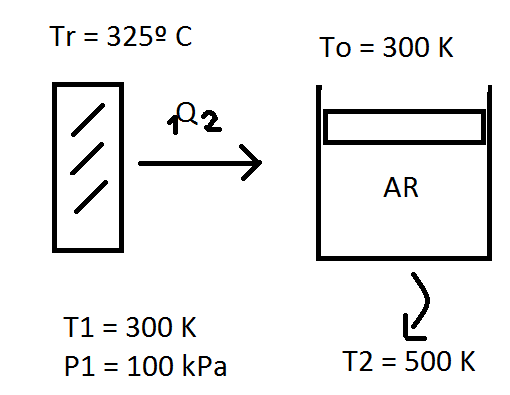
\includegraphics[scale=0.58]{./fig/3.png}
\caption{\label{fig:3}3} 
\end{center}
\end{figure}
\begin{itemize}
\item	a) $W=?$
\item	b) $q=?$
\item	c) $s_{ger}=?$

\end{itemize}

\subsection*{Soluçao}

\paragraph*{Hipóteses}
\begin{itemize}
\item $c_{P}$ constante
\item $Pv = RT$
\item $PV^{n}=cte, n = 1.3$
\end{itemize}

\subsubsection*{item a}
trabalho específico:
\[w _{1 \rightarrow 2}= \frac{P_{2}v_{2}-P_{1}v_{1}}{1-n}\]
\[w _{1 \rightarrow 2}= \frac{R(T_{2}-T_{1})}{1-n}\]
\[w _{1 \rightarrow 2}= -191.3 \ kJ/kg\]
\subsubsection*{item b}
\[q _{1 \rightarrow 2}= u_{2}-u_{1}+w _{1 \rightarrow 2}\]
\[q _{1 \rightarrow 2}=c_{V}(T_{2}-T_{1})+w _{1 \rightarrow 2}\]
\[q _{1 \rightarrow 2}=-48.03 kJ/kg\]
\subsubsection*{item c}
\[s_{ger}=(s_{2}-s_{1})-\frac{q _{1 \rightarrow 2}}{T_{0}}=0.0037\ kJ/kg\]
\[s_{2}-s_{1}=c_{p}\ln(\frac{T_{2}}{T_{1}})-R\ln(\frac{P_{2}}{P_{1}})\]
\newpage
\section{ Ex 8.117  6ª Ed.}

\begin{figure}[h]
\begin{center}
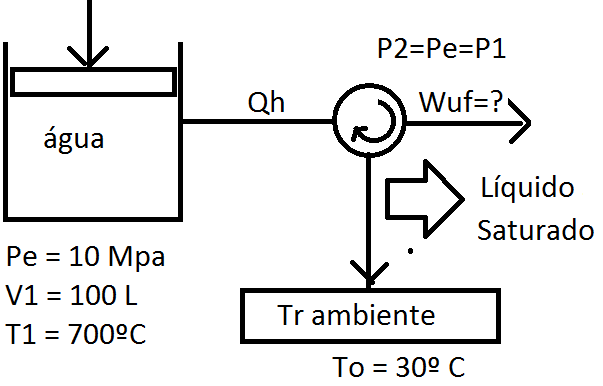
\includegraphics[scale=0.68]{./fig/4.png}
\caption{\label{fig:4}4} 
\end{center}
\end{figure}




\subsection*{Soluçao}

\begin{figure}[h]
\begin{center}
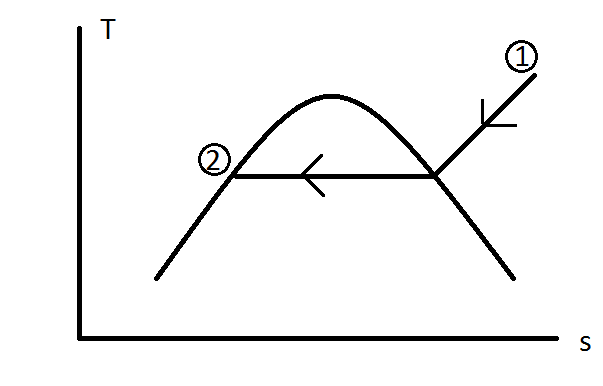
\includegraphics[scale=0.38]{./fig/5.png}
\caption{\label{fig:4}5} 
\end{center}
\end{figure}

Sistema:  água\\\ 1ª Lei: 
\[Q_{1 \rightarrow 2}=m(u_{2}-u_{1})+W_{e}\]
\[W_{e}=P_{e}(v_{2}-v_{1})m=-966.7kJ\]
\begin{itemize}
\item m = 2.294kg
\item $v_{2}=0.001452\ m^{3}/kg$
\item $v_{1}=0.04359\ m^{3}/kg$
\item $u_{1}=3433\ kJ/kg$
\item $u_{2}=1393\ kJ/kg$
\[Q_{1 \rightarrow 2}=-5647\ kJ\]
\paragraph*{Processo Global Reversível}
\[\Delta S_{eq}=0\]
\[\Delta S_{eq}=\Delta S_{SIST}+\Delta S_{MEIO}\]
\[\Delta S_{SIST}=m(s_{2}-s_{1})\]
\[\Delta S_{MEIO}=-\frac{Q_{2}}{T_{0}}\]

\end{itemize}



\end{document}